\documentclass[a4paper]{article}

\usepackage[UTF8]{ctex}
\usepackage[a4paper,margin=1in]{geometry}
\usepackage{graphicx}
\usepackage{float}
\usepackage{listings}
\usepackage{longtable}
\usepackage{booktabs}
\usepackage{hyperref}
\usepackage{fancyhdr}
\usepackage{lastpage}
\usepackage{color}
\usepackage{xcolor}
\usepackage{indentfirst}        % 首段缩进
\setlength{\parindent}{2em}     % 缩进2字符
\usepackage{zhnumber}           % 中文编号
\usepackage[dvipsnames]{xcolor}
\usepackage{amsmath}
\usepackage{multimedia}  % 添加多媒体支持
\usepackage{qrcode}      % 添加二维码支持(可选)
\usepackage[most]{tcolorbox}  % 添加彩色框支持
%\newcommand{\college}{中山大学计算机学院}
\newcommand{\projname}{计算机图形学|作业一}
\newcommand{\reporttitle}{基于OpenGL的字母绘制实验}
\newcommand{\stuno}{23336179}
\newcommand{\authorname}{马福泉}
\newcommand{\major}{计算机科学与技术}
\newcommand{\adviser}{陶钧}
\newcommand{\startdate}{2025年10月20日}
\newcommand{\labenddate}{2025年11月7日}
\newcommand{\labroom}{B402}

\pagestyle{fancy} % 使用 fancyhdr 风格
\fancyhf{}      % 清空默认的页眉页脚

% 设置页眉
\fancyhead[L]{\kaishu \projname}      % 左侧页眉显示项目名称
\fancyhead[C]{\kaishu \reporttitle}    % 中间页眉显示报告标题
\fancyhead[R]{\kaishu \authorname} % 右侧页眉显示作者姓名

% 设置页脚
\fancyfoot[C]{第 \thepage 页，共 \pageref{LastPage} 页} % 中间页脚显示页码

% 去除页眉页脚与正文之间的分隔线
\renewcommand{\headrulewidth}{0.4pt}
\renewcommand{\footrulewidth}{0pt}

% 设置文档背景颜色
\definecolor{mybgcolor}{RGB}{0, 0, 0} % 定义背景颜色
\definecolor{NavyBlue}{RGB}{0,0,128} % 添加颜色定义
% \pagecolor{mybgcolor} % 设置背景颜色

\lstset{
    basicstyle=\ttfamily\small,
    commentstyle=\color{gray},
    keywordstyle=\color{blue},
    stringstyle=\color{red},
    breaklines=true,
    frame=single,
    numbers=left,
    numberstyle=\tiny\color{gray},
    tabsize=4,
    showstringspaces=false,
    captionpos=b,
    escapeinside={\%}{\%},
    language=C++
}

\begin{document}

% 封面
\begin{titlepage}
    \centering
    

    
\includegraphics[width=10cm]{img/SYSULogo.png}

    \vspace{1em}
    %{\Large \college \par}
    \vspace{1em}
    {\Large \kaishu \projname \par}
    \vspace{3em}

    

    
    {\fontsize{40pt}{42pt}\kaishu \selectfont \boldmath \reporttitle\par}
    \vspace*{\fill}

    \begin{center}
    {\Large
    \makebox[5em][s]{学号}:\underline{\makebox[15em][c]{\kaishu \stuno}}\\[1em]
    \makebox[5em][s]{姓名}:\underline{\makebox[15em][c]{\kaishu \authorname}}\\[1em]
    \makebox[5em][s]{专业}:\underline{\makebox[15em][c]{\kaishu \major}}\\[1em]
    \makebox[5em][s]{指导教师}:\underline{\makebox[15em][c]{\kaishu \adviser}}\\[1em]
    \makebox[5em][s]{起始日期}:\underline{\makebox[15em][c]{\kaishu \startdate}}\\[1em]
    \makebox[5em][s]{结束日期}:\underline{\makebox[15em][c]{\kaishu \labenddate}}\\[1em]
    \makebox[5em][s]{实验地点}:\underline{\makebox[15em][c]{\kaishu \labroom}}
    }
    \end{center}

    \vspace*{\fill}
\end{titlepage}

% 目录
\tableofcontents
\newpage

% 实验报告正文开始

\section{实验概述}

\subsection{实验目的}
本实验旨在通过OpenGL环境搭建和基本图形绘制，掌握计算机图形学中的基础概念和实现方法。具体包括：
\begin{enumerate}
    \item 掌握OpenGL开发环境的搭建过程
    \item 理解OpenGL基本图元的使用方法
    \item 学会在二维平面绘制复杂图形
    \item 掌握三维图形绘制和变换操作
    \item 比较不同投影方式和绘制方法的差异
\end{enumerate}

\subsection{实验内容}
1. 环境搭建：
\begin{enumerate}
    \item[(1)] 要求在实验报告中详细描述环境搭建过程、中间遇到的困难及问题的解决方案。
    \item[(2)] 建议超算习堂模板中的环境配置教程完成实验环境搭建和调试，请尽量按照教程中的环节搭建，以方便统一作业批改环境。
    \item[(3)] 若使用其他方法搭建环境并实现作业内容，请给出详细的程序运行说明文档。
\end{enumerate}

2. 绘制平面姓名首字母：
\begin{enumerate}
    \item[(1)] 基本要求：
    \begin{itemize}
        \item 在二维画布（$x$平面）上，使用基本图元（三角形），以原点为绘制中心，绘制自己姓名首字母（绘制结果参考图 1）。
    \end{itemize}
    \item[(2)] 字母选取要求：
    \begin{itemize}
        \item 当名字为两字时，需补一个顺位字母，例如姓名首字母为 LS，则需要绘制 LST 三个字母；
        \item 当名字大于三字时，取前三个字的首字母即可；
        \item 当名字中存在相同首字母时，将第二个相同的字母替换为顺位字母，例如姓名首字母为 LL，则需要绘制 LMN；
        \item 当姓名首字母中重复的字母为 Z 时，取循环顺位字母 A。
    \end{itemize}
    \item[(3)] 讨论：
    \begin{itemize}
        \item 比较 GL\_TRIANGLES, GL\_TRIANGLE\_STRIP, GL\_QUADS, GL\_QUAD\_STRIP 的绘制开销（需要的 glVertex 调用次数）；
        \item 比较以下两个视角下，Orthogonal 及 Perspective 投影方式产生的图像：
        \begin{enumerate}
            \item 从（0,0,d）看向原点(0, 0, 0)；
            \item 从(0, 0.5*d, d)看向原点(0, 0, 0)。
        \end{enumerate}
        注：可使用(0, 1, 0)作为视角的上方向（up）。
    \end{itemize}
    \item 图 1 二维字母绘制图例见下图：
    \begin{figure}[H]
        \centering
        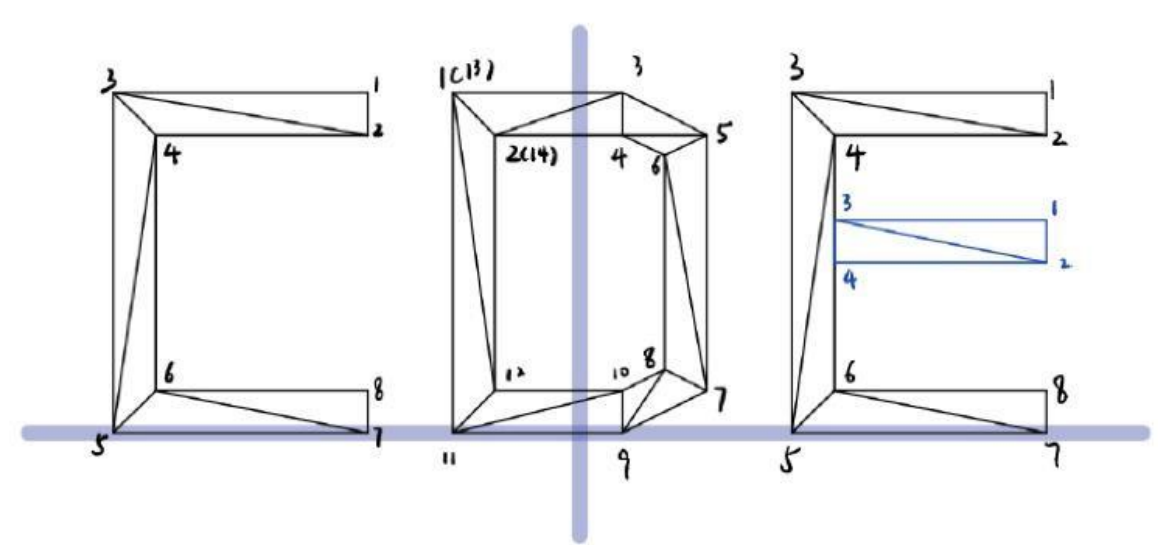
\includegraphics[width=0.6\textwidth]{img/example.png}
        \caption{二维字母绘制图例}
        \label{fig:example}
    \end{figure}
\end{enumerate}

3. 绘制立体姓氏首字母：
\begin{enumerate}
    \item[(1)] 基本要求：
    \begin{itemize}
        \item 在三维空间内，以原点为绘制中心，绘制立体的姓氏首字母。
    \end{itemize}
    \item[(2)] 绘制要求：
    \begin{itemize}
        \item 若姓氏大于一字，取第一字的首字母；
        \item 要求在 xoy 平面绘制字母的 2D 样式，并在 z 轴上增加字母厚度以达到立体效果，此处厚度不做要求、可自定义。
    \end{itemize}
    \item[(3)] 实现内容：
    \begin{itemize}
        \item 分别实现并比较字母绕 x、y、z 轴的旋转；
        \item 旋转的方式不作限制，若有多种旋转方式，可对比旋转方式，比如以 x 轴为旋转轴顺时针旋转和以 x 轴为旋转轴逆时针旋转的对比。
    \end{itemize}
\end{enumerate}

\section{环境搭建}

1. 安装Visual Studio和CMake

Visual Studio（下称VS）一般选择2022版本，下载链接见\url{https://visualstudio.microsoft.com/zh-hans/}。  
安装组件时，查阅资料安装了以下工作负载和单个组件：

\begin{itemize}
    \item 使用C++的游戏开发：计算机图形学开发必备，包含创建3D图形、游戏引擎等所需的核心C++工具。
    \item 使用C++的桌面开发：提供额外工具和示例，使用Clang/LLVM工具集构建时必需。
    \item .NET桌面开发：如项目涉及.NET桌面应用可选安装。
    \item C++分析工具：有助于代码质量和性能优化。
    \item C++ AddressSanitizer：用于检测内存错误（可选）。
    \item Windows 10或11 SDK（10.0.18362或更高版本）：提供Windows系统级API和功能支持。
    \item HLSL工具：用于编写和调试着色器（如涉及DirectX开发）。
    \item 面向Unreal引擎的IDE支持：如使用Unreal引擎开发需勾选。
\end{itemize}

安装完成截图如下：

\begin{figure}[H]
    \centering
    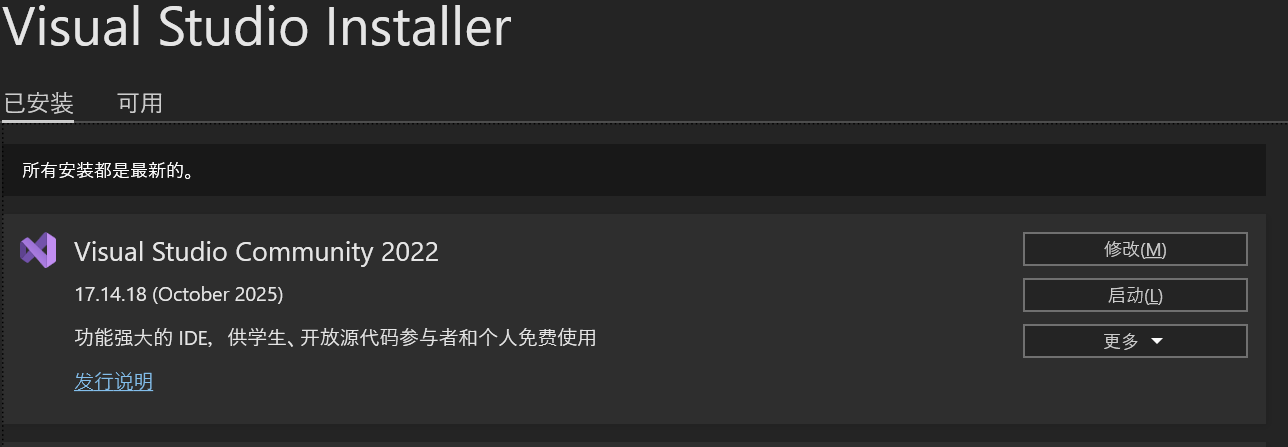
\includegraphics[width=0.7\textwidth]{img/vs_success.png}
    \caption{Visual Studio安装成功截图}
\end{figure}

CMake下载见\url{https://cmake.org/download/}，安装的版本为cmake-4.2.0-rc1。  
安装成功截图如下：

\begin{figure}[H]
    \centering
    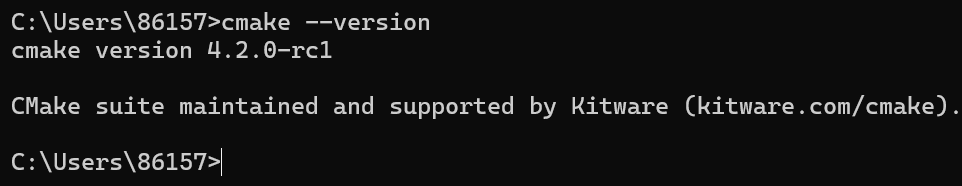
\includegraphics[width=0.7\textwidth]{img/cmake_success.png}
    \caption{CMake安装成功截图}
\end{figure}

2. 写CMakeLists.txt

选定一个空文件夹作为项目根目录，在该文件夹中新建CMakeLists.txt文件，并将文档提供内容复制进去。

3. 写cpp文件

在项目根目录创建src文件夹，在src文件夹中创建main.cpp文件，填入文档所给内容，用于测试环境是否配置成功。

4. CMake构建

在项目文件夹根目录（CMakeLists.txt所在目录）打开终端（如CMD、Powershell等），依次输入如下命令：

\begin{verbatim}
mkdir build
cd build
cmake ..
cmake --build .
\end{verbatim}

构建结果截图如下：

\begin{figure}[H]
    \centering
    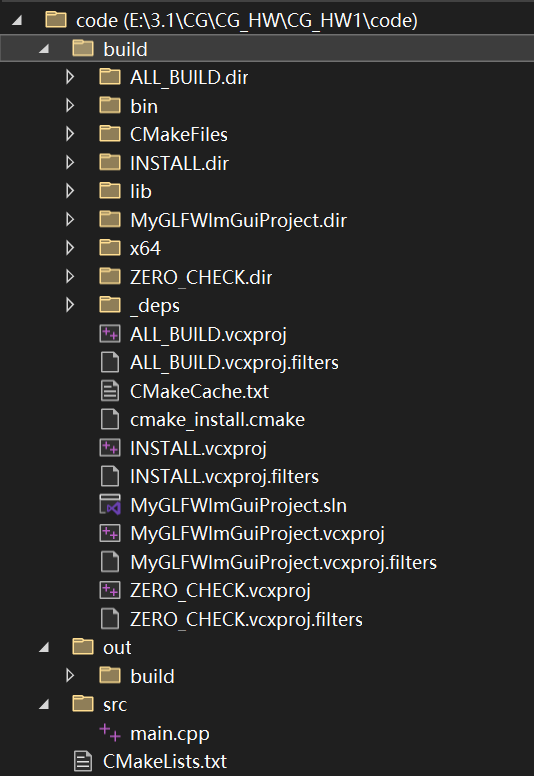
\includegraphics[width=0.7\textwidth]{img/build.png}
    \caption{CMake构建成功截图}
\end{figure}

5. 用Visual Studio打开项目文件夹

进入Visual Studio界面，点击“打开本地文件夹”，选择CMakeLists.txt所在的文件夹。稍等片刻，VS会自动根据CMakeLists.txt配置项目。  
运行测试代码，在VS左侧窗口中，双击src中的main.cpp打开并运行。

运行成功截图如下：

\begin{figure}[H]
    \centering
    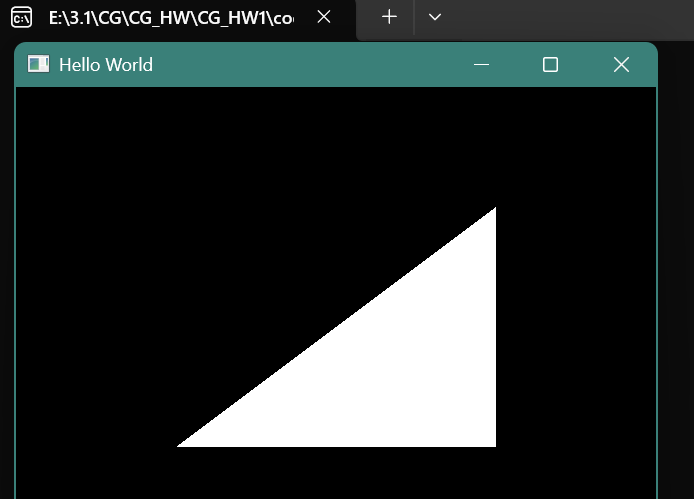
\includegraphics[width=0.4\textwidth]{img/test1.png}
    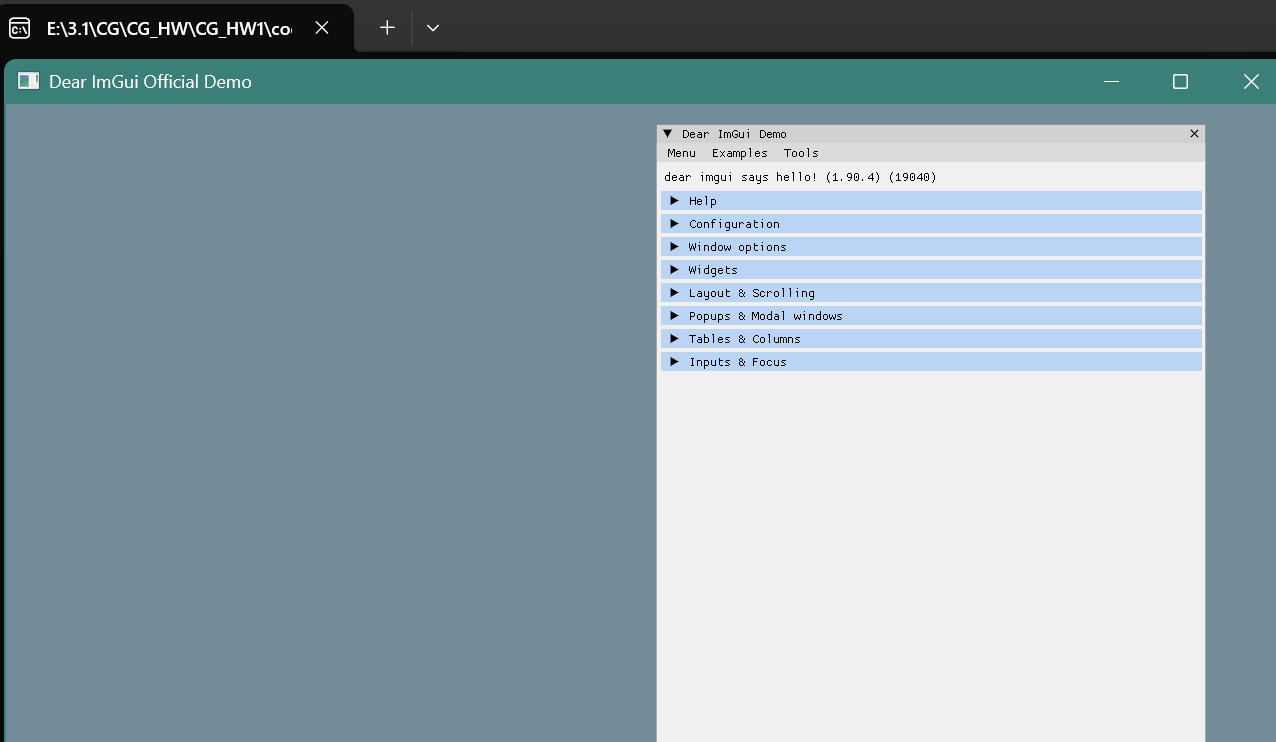
\includegraphics[width=0.5\textwidth]{img/test2.png}
    \caption{测试代码运行成功截图}
\end{figure}

\section{二维字母绘制}

\subsection{字母选取规则}

根据作业要求，我的姓名为"马福泉"，首字母为MFQ。由于是三个字，直接取前三个字的首字母即可。

\subsection{绘制思路}

使用OpenGL的三角形图元（GL\_TRIANGLES）来构建字母。每个字母都通过多个三角形组合而成：
\begin{itemize}
    \item 字母M：由8个三角形组成
    \item 字母F：由6个三角形组成  
    \item 字母Q：由11个三角形组成
\end{itemize}

\subsection{核心代码实现}

\begin{lstlisting}[caption={MFQ字母顶点定义与绘制（纵坐标为0）}]
const int letterM[] = {
    0, 0, 0, 0, 7, 0, 1, 0, 0,
    1, 0, 0, 0, 7, 0, 1, 5, 0,
    0, 7, 0, 1, 5, 0, 3, 4, 0,
    1, 5, 0, 3, 4, 0, 3, 3, 0,
    3, 4, 0, 3, 3, 0, 5, 5, 0,
    3, 4, 0, 5, 5, 0, 6, 7, 0,
    5, 0, 0, 5, 5, 0, 6, 7, 0,
    5, 0, 0, 6, 7, 0, 6, 0, 0
};

const int letterF[] = {
    8, 0, 0, 8, 6, 0, 9, 0, 0,
    9, 0, 0, 8, 6, 0, 9, 6, 0,
    8, 6, 0, 13, 6, 0, 8, 7, 0,
    8, 7, 0, 13, 6, 0, 13, 7, 0,
    9, 3, 0, 12, 3, 0, 9, 4, 0,
    9, 4, 0, 12, 3, 0, 12, 4, 0
};

const int letterQ[] = {
    20, 0, 0, 19, 1, 0, 21, 1, 0,
    16, 1, 0, 21, 1, 0, 20, 2, 0,
    15, 2, 0, 16, 1, 0, 20, 2, 0,
    15, 2, 0, 17, 2, 0, 15, 4, 0,
    20, 2, 0, 18, 2, 0, 20, 4, 0,
    16, 3, 0, 15, 4, 0, 16, 5, 0,
    19, 3, 0, 20, 4, 0, 19, 5, 0,
    15, 4, 0, 15, 6, 0, 17, 6, 0,
    20, 4, 0, 20, 6, 0, 18, 6, 0,
    15, 6, 0, 20, 6, 0, 16, 7, 0,
    16, 7, 0, 19, 7, 0, 20, 6, 0
};

// 绘制函数示例
void drawLetter(const int* vertices, int triangleCount) {
    glBegin(GL\textunderscore TRIANGLES);
    for (int i = 0; i < triangleCount * 9; i += 3) {
        glVertex3i(vertices[i], vertices[i + 1], vertices[i + 2]);
    }
    glEnd();
}

// 使用方法：
// drawLetter(letterM, 8);
// drawLetter(letterF, 6);
// drawLetter(letterQ, 11);
\end{lstlisting}

\subsection{绘制结果}

% 此处添加2D字母绘制结果图
\begin{figure}[H]
    \centering
    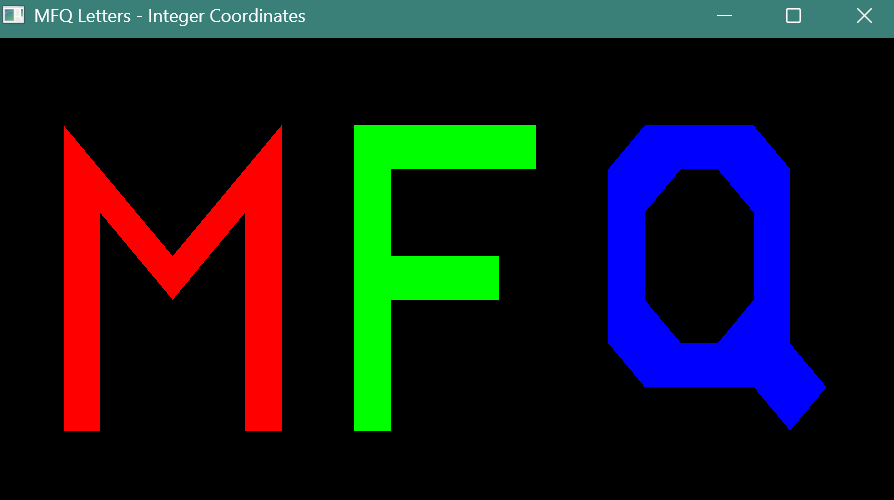
\includegraphics[width=0.8\textwidth]{img/2d_letters.png}
    \caption{二维字母MFQ绘制结果}
    \label{fig:2d_letters}
\end{figure}

\subsection{讨论一：不同绘制方式的开销比较}

在绘制字母M、F、Q时，我们可以使用不同的OpenGL图元类型。下面分析各种图元类型的特点及其绘制开销：

\subsubsection{图元类型分析}

\begin{itemize}
    \item \textbf{GL\_TRIANGLES}：独立三角形模式，每3个顶点构成一个三角形，顶点不共享。这是最基础的绘制方式，灵活性高但顶点数据冗余较多。
    
    \item \textbf{GL\_TRIANGLE\_STRIP}：三角形条带模式，除前两个顶点外，每增加一个顶点就形成一个新三角形。相邻三角形共享边，大大减少了顶点数量。
    
    \item \textbf{GL\_QUADS}：独立四边形模式，每4个顶点构成一个四边形。适合绘制矩形区域，但现代OpenGL已不推荐使用。
    
    \item \textbf{GL\_QUAD\_STRIP}：四边形条带模式，除前两个顶点外，每增加2个顶点就形成一个新四边形。相邻四边形共享边。
\end{itemize}

\subsubsection{具体开销计算}
M、F、Q的设计图如下：

\begin{figure}[H]
    \centering
    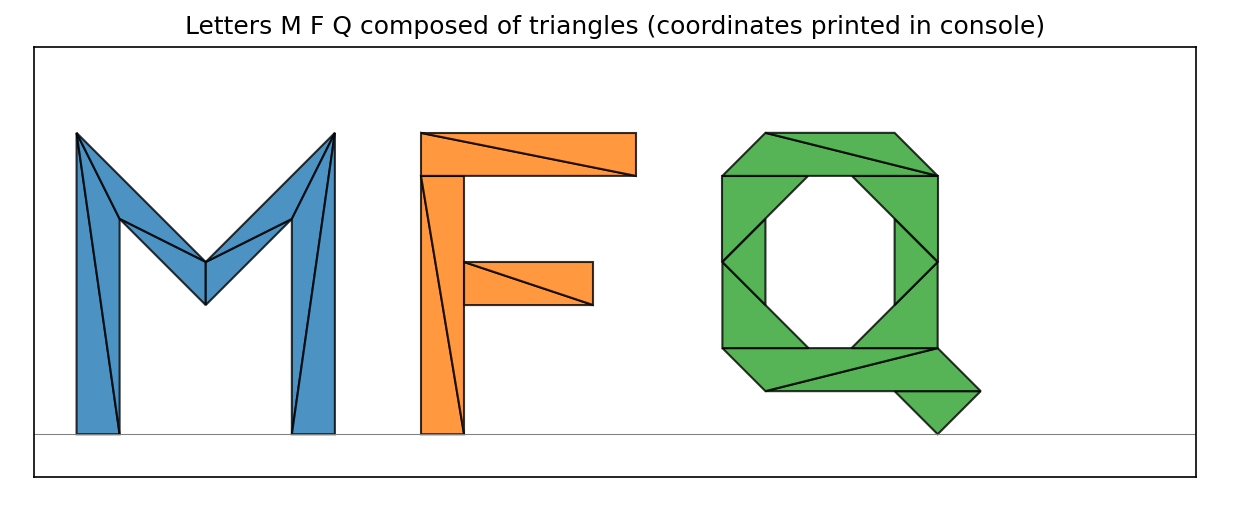
\includegraphics[width=0.8\textwidth]{img/design.png}
    \caption{M、F、Q的设计图}
    \label{fig:design_letters}
\end{figure}

根据字母M、F、Q的设计图，各图元类型的绘制开销如下：

\begin{table}[H]
\centering
\caption{不同图元类型的绘制开销比较}
\begin{tabular}{|l|c|c|c|}
\hline
绘制方式 & 字母分解数量 & 总顶点调用次数 & 效率排名 \\
\hline
GL\_TRIANGLES & M(8)+F(6)+Q(11)=25个三角形 & $25 \times 3 = 75$ & 4 \\
GL\_TRIANGLE\_STRIP & M(10)+F(10)+Q(18)个顶点 & $10+10+18 = 38$ & 2 \\
GL\_QUADS & M(4)+F(3)+Q(9)=16个四边形 & $16 \times 4 = 64$ & 3 \\
GL\_QUAD\_STRIP & M(10)+F(10)+Q(16)个顶点 & $10+10+16 = 36$ & 1 \\
\hline
\end{tabular}
\label{tab:draw_cost}
\end{table}

\subsubsection{结果分析}

从计算结果可以看出：

\begin{enumerate}
    \item \textbf{GL\_QUAD\_STRIP效率最高}：仅需36次glVertex调用，因为相邻四边形共享边，大大减少了顶点重复。
    
    \item \textbf{GL\_TRIANGLE\_STRIP次之}：需要38次glVertex调用，三角形条带模式有效减少了顶点冗余。
    
    \item \textbf{GL\_QUADS排第三}：需要64次glVertex调用，虽然四边形更适合描述矩形字母结构，但缺乏顶点共享机制。
    
    \item \textbf{GL\_TRIANGLES效率最低}：需要75次glVertex调用，每个三角形都需要完整的3个顶点，顶点重复最多。
\end{enumerate}

\textbf{注意}：虽然GL\_QUAD相关的图元在某些场景下效率较高，但在现代OpenGL（3.0+）中已被弃用，建议使用三角形图元配合索引缓冲区来实现高效绘制。

\subsection{讨论二：投影方式比较}

\subsubsection{投影原理分析}

在计算机图形学中，投影变换是将三维场景映射到二维屏幕的关键步骤。主要有两种投影方式：

\begin{itemize}
    \item \textbf{正交投影（Orthogonal Projection）}：平行投影，物体的大小不随距离变化而改变，保持平行线的平行性。适用于工程制图、建筑图纸等需要精确尺寸的场合。
    
    \item \textbf{透视投影（Perspective Projection）}：中心投影，模拟人眼观察效果，远处的物体看起来更小，产生景深效果。符合人类视觉习惯，常用于游戏和动画渲染。
\end{itemize}

\subsubsection{实验设置}

本实验比较了以下四种视角组合下的投影效果：

\begin{enumerate}
    \item \textbf{视角1 + 正交投影}：从(0,0,d)看向原点(0,0,0)，使用正交投影
    \item \textbf{视角1 + 透视投影}：从(0,0,d)看向原点(0,0,0)，使用透视投影
    \item \textbf{视角2 + 正交投影}：从(0,0.5*d,d)看向原点(0,0,0)，使用正交投影
    \item \textbf{视角2 + 透视投影}：从(0,0.5*d,d)看向原点(0,0,0)，使用透视投影
\end{enumerate}

其中，d=5.0，上方向向量为(0,1,0)。

\subsubsection{四种视角透视的区别分析}

\textbf{1. 视角1正交投影}
\begin{itemize}
    \item 观察角度：正视角度（沿z轴负方向观察）
    \item 投影特点：字母保持原始比例，无透视变形
    \item 视觉效果：类似于工程图纸，所有平行线保持平行
    \item 适用场景：技术制图、精确测量
\end{itemize}

\textbf{2. 视角1透视投影}
\begin{itemize}
    \item 观察角度：正视角度（沿z轴负方向观察）
    \item 投影特点：字母中心区域与边缘区域有轻微的透视差异
    \item 视觉效果：更加真实自然，符合人眼观察习惯
    \item 适用场景：游戏渲染、虚拟现实
\end{itemize}

\textbf{3. 视角2正交投影}
\begin{itemize}
    \item 观察角度：斜视角度（从上方偏移位置观察）
    \item 投影特点：字母形状发生倾斜，但保持平行投影特性
    \item 视觉效果：类似于等轴测图，可同时观察到多个面
    \item 适用场景：建筑设计、机械制图的轴测图
\end{itemize}

\textbf{4. 视角2透视投影}
\begin{itemize}
    \item 观察角度：斜视角度（从上方偏移位置观察）
    \item 投影特点：字母既有倾斜又有透视变形，最接近真实观察效果
    \item 视觉效果：最强的三维立体感和空间深度感
    \item 适用场景：3D游戏、电影特效、虚拟现实应用
\end{itemize}

\subsubsection{代码要点展示}

在OpenGL中实现不同投影方式的关键代码片段：

\begin{lstlisting}[caption={投影矩阵设置}]
// 正交投影设置
void setOrthogonalProjection() {
    glMatrixMode(GL\textunderscore PROJECTION);
    glLoadIdentity();
    glOrtho(-2.0, 2.0, -2.0, 2.0, 1.0, 10.0);
}

// 透视投影设置
void setPerspectiveProjection() {
    glMatrixMode(GL\textunderscore PROJECTION);
    glLoadIdentity();
    gluPerspective(45.0, 1.0, 1.0, 10.0);
}

// 视角设置
void setViewpoint(int viewType) {
    glMatrixMode(GL\textunderscore MODELVIEW);
    glLoadIdentity();
    
    if(viewType == 1) {
        // 视角1：从(0,0,5)看向原点
        gluLookAt(0.0, 0.0, 5.0,    // 眼睛位置
                  0.0, 0.0, 0.0,    // 目标位置
                  0.0, 1.0, 0.0);   // 上方向
    } else {
        // 视角2：从(0,2.5,5)看向原点
        gluLookAt(0.0, 2.5, 5.0,    // 眼睛位置
                  0.0, 0.0, 0.0,    // 目标位置
                  0.0, 1.0, 0.0);   // 上方向
    }
}
\end{lstlisting}

\subsubsection{实验结果对比}

投影方式比较的实验结果如下图所示：

\begin{figure}[H]
    \centering
    
\includegraphics[width=0.45\textwidth]{img/ortho_view1.png}
    
\includegraphics[width=0.45\textwidth]{img/persp_view1.png}
    \caption{视角1下的正交投影（左）和透视投影（右）比较}
    \label{fig:projection_view1}
\end{figure}

\begin{figure}[H]
    \centering
    
\includegraphics[width=0.45\textwidth]{img/ortho_view2.png}
    
\includegraphics[width=0.45\textwidth]{img/persp_view2.png}
    \caption{视角2下的正交投影（左）和透视投影（右）比较}
    \label{fig:projection_view2}
\end{figure}

\subsubsection{结论分析}

通过对比实验可以得出：
\begin{enumerate}
    \item \textbf{正交投影}适合需要精确尺寸的技术应用，但缺乏真实感
    \item \textbf{透视投影}提供更真实的视觉效果，适合交互式图形应用
    \item \textbf{视角变化}对投影效果有显著影响，斜视角度能够提供更丰富的空间信息
    \item \textbf{投影方式选择}应根据具体应用需求确定：工程制图选择正交投影，游戏渲染选择透视投影
\end{enumerate}

\section{三维字母绘制}
\subsection{立体字母设计}
根据要求，绘制姓氏"马"的首字母"M"的立体版本。设计思路：
\begin{enumerate}
    \item 在xoy平面绘制字母M的2D轮廓
    \item 沿z轴方向拉伸，增加厚度
    \item 添加前后面和侧面，形成完整的立体效果
\end{enumerate}

\subsection{核心实现代码}
\begin{lstlisting}[caption={3D字母M数据结构定义}]
// 3D顶点结构
struct Vertex {
    float x, y, z;
    Vertex(float x, float y, float z) : x(x), y(y), z(z) {}
};

// 三角形结构
struct Triangle {
    Vertex v1, v2, v3;
    Triangle(Vertex v1, Vertex v2, Vertex v3) : v1(v1), v2(v2), v3(v3) {}
};

// 立体字母M的三角形集合
std::vector<Triangle> letterM3D;
const float THICKNESS = 2.0f;  // 厚度参数
\end{lstlisting}

\begin{lstlisting}[caption={多模式旋转系统}]
// 旋转参数
float angleX = 0.0f, angleY = 0.0f, angleZ = 0.0f;
int rotationAxis = 0; // 0:x, 1:y, 2:z, 3:组合旋转

// 旋转更新逻辑
if (autoRotate) {
    switch (rotationAxis) {
        case 0: angleX += rotationSpeed; break;          // X轴旋转
        case 1: angleY += rotationSpeed; break;          // Y轴旋转  
        case 2: angleZ += rotationSpeed; break;          // Z轴旋转
        case 3: // 组合旋转
            angleX += rotationSpeed;
            angleY += rotationSpeed * 0.7f;
            angleZ += rotationSpeed * 0.3f;
            break;
    }
}

// 应用旋转变换
glRotatef(angleX, 1.0f, 0.0f, 0.0f);
glRotatef(angleY, 0.0f, 1.0f, 0.0f);
glRotatef(angleZ, 0.0f, 0.0f, 1.0f);
\end{lstlisting}

\subsection{代码使用说明}
\subsubsection{键盘控制说明}
\begin{itemize}
    \item \textbf{X/Y/Z键}：分别启动绕X、Y、Z轴的自动旋转
    \item \textbf{A键}：启动XYZ组合旋转模式
    \item \textbf{R键}：重置所有旋转角度到初始状态
    \item \textbf{空格键}：切换自动旋转和手动旋转模式
    \item \textbf{+/-键}：动态调整旋转速度
    \item \textbf{方向键}：手动模式下控制X、Y轴旋转
    \item \textbf{Q/E键}：手动模式下控制Z轴旋转
\end{itemize}

\subsection{代码亮点介绍}

\subsubsection{1. 自动化立体建模算法}
实现了从2D轮廓到3D立体的转换：
\begin{itemize}
    \item \textbf{前后表面生成}：自动从2D顶点生成前表面，并通过Z轴偏移创建后表面
    \item \textbf{智能侧面构建}：自动识别2D轮廓的边缘，生成连接前后表面的侧面三角形
    \item \textbf{法线方向处理}：后表面顶点顺序自动反转，确保正确的面法线方向
\end{itemize}

\subsubsection{2. 多模式旋转系统}
实现了多种旋转模式：
\begin{itemize}
    \item \textbf{单轴旋转}：绕X、Y、Z轴的独立旋转，便于观察各轴旋转效果
    \item \textbf{组合旋转}：三轴同时旋转但速度不同，创造复杂的3D运动轨迹
    \item \textbf{自动/手动切换}：支持自动播放和手动精确控制两种模式
    \item \textbf{动态速度调节}：实时调整旋转速度，满足不同观察需求
\end{itemize}

\subsubsection{3. 颜色区分}
基于几何特征的智能着色系统：
\begin{itemize}
    \item \textbf{自动面识别}：根据顶点Z坐标自动判断前表面、后表面和侧面
    \item \textbf{差异化着色}：前表面（红色）、后表面（蓝色）、侧面（绿色）
    \item \textbf{立体感增强}：不同颜色有助于用户更好地理解3D结构
\end{itemize}

\subsubsection{4. 用户体验优化}
注重交互体验的细节设计：
\begin{itemize}
    \item \textbf{防抖处理}：空格键切换时避免连续触发
    \item \textbf{边界保护}：旋转速度调节有下限保护
    \item \textbf{实时反馈}：控制台输出详细的操作说明
    \item \textbf{状态可视化}：不同旋转模式有明显的视觉区别
\end{itemize}

\subsection{结果展示}

\begin{figure}[H]
    \centering
    
\includegraphics[width=0.6\textwidth]{img/3d_letter_static.png}
    \caption{静态3D字母M展示}
    \label{fig:3d_static}
\end{figure}

\subsubsection{X轴旋转效果}

字母M绕X轴旋转的关键帧序列展示旋转过程:

\begin{figure}[H]
    \centering
    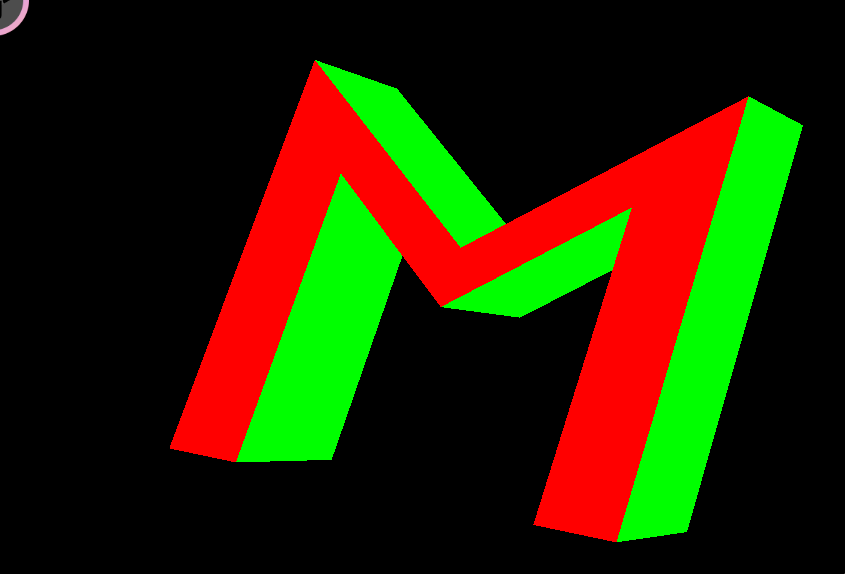
\includegraphics[width=0.4\textwidth]{img/rotate_x1.png}
    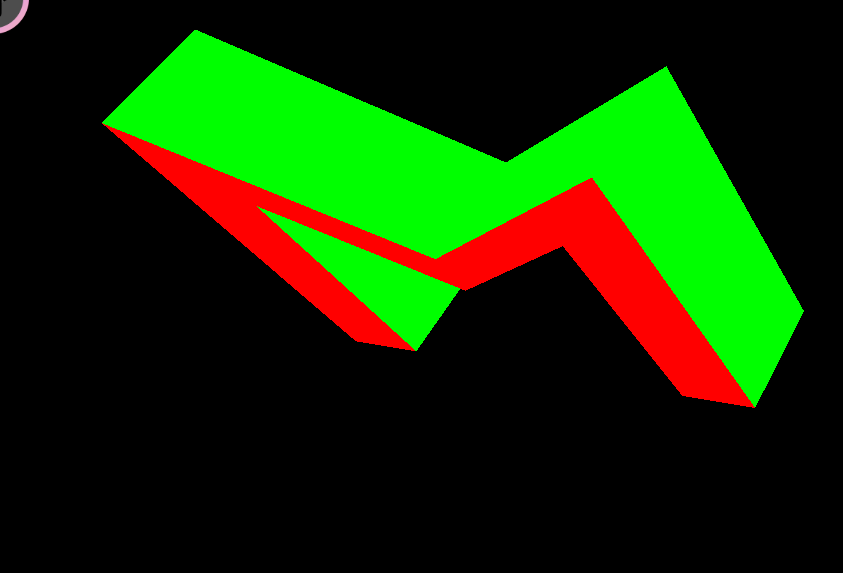
\includegraphics[width=0.4\textwidth]{img/rotate_x2.png}
    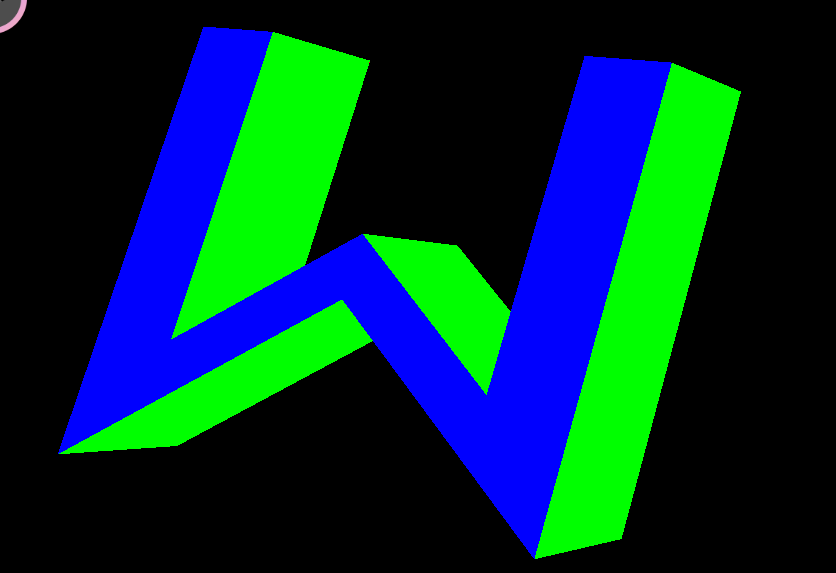
\includegraphics[width=0.4\textwidth]{img/rotate_x3.png}
    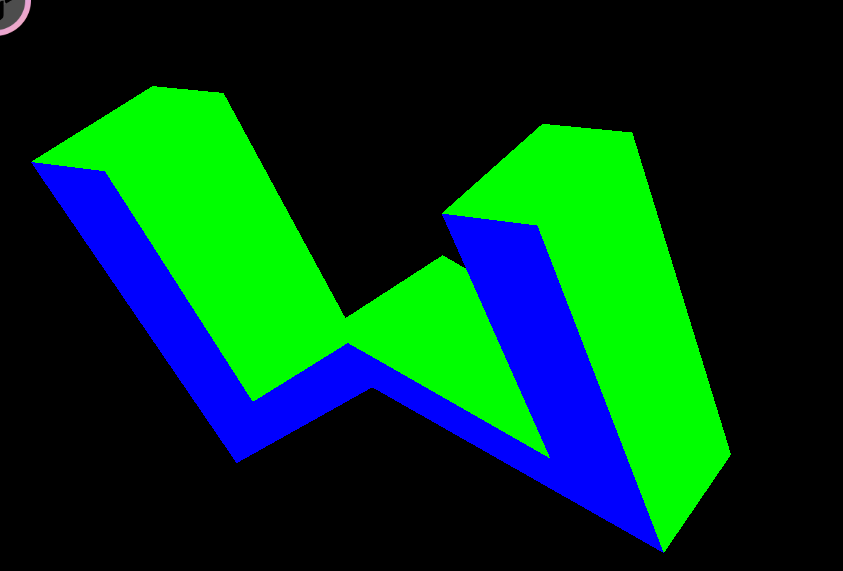
\includegraphics[width=0.4\textwidth]{img/rotate_x4.png}
    \caption{绕X轴旋转关键帧}
    \label{fig:rotation_x}
\end{figure}

\subsubsection{Y轴旋转效果}

字母M绕Y轴旋转的关键帧序列展示旋转过程:

\begin{figure}[H]
    \centering
    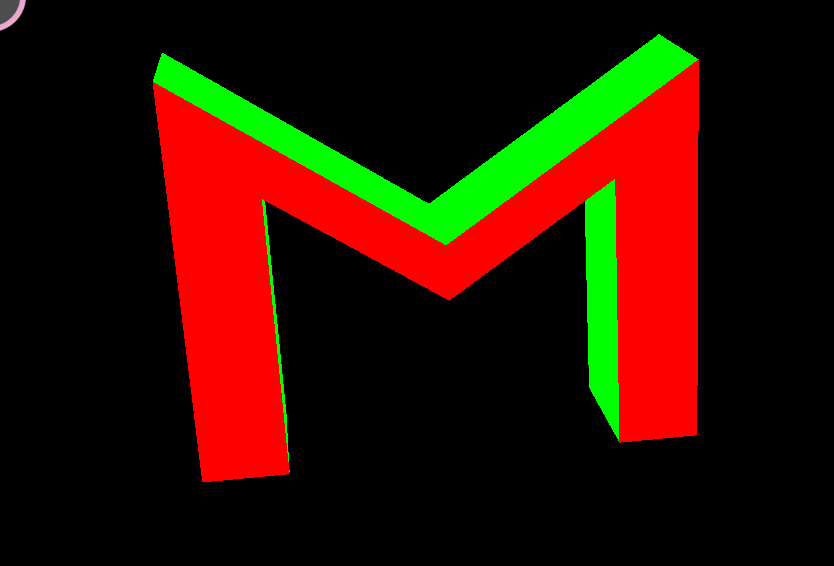
\includegraphics[width=0.4\textwidth]{img/rotate_y1.png}
    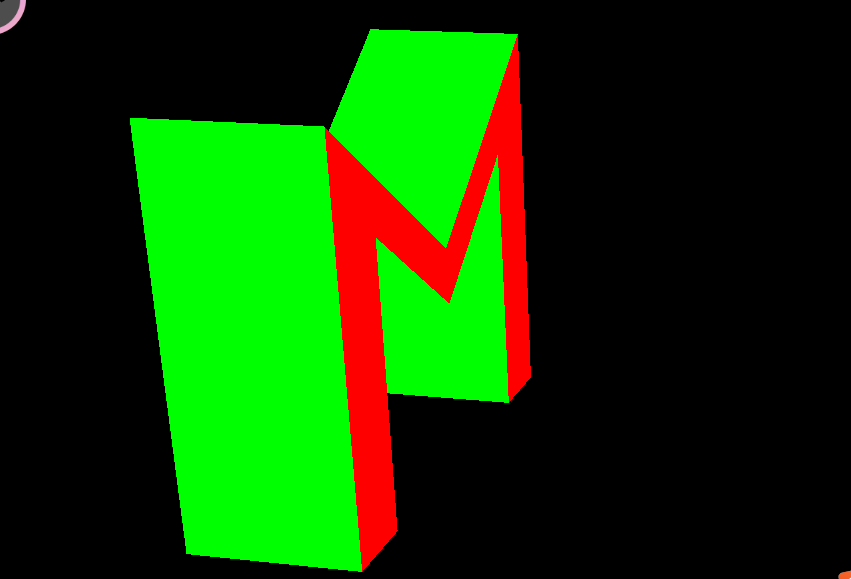
\includegraphics[width=0.4\textwidth]{img/rotate_y2.png}
    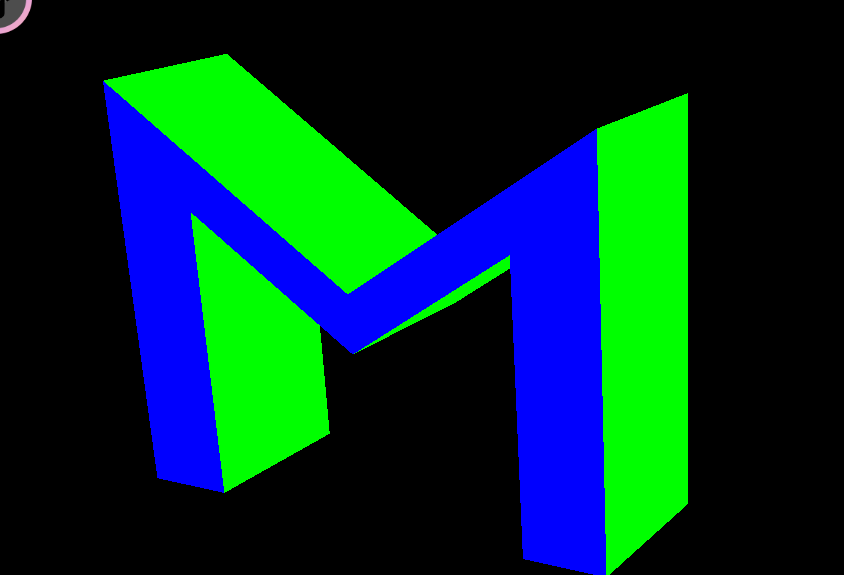
\includegraphics[width=0.4\textwidth]{img/rotate_y3.png}
    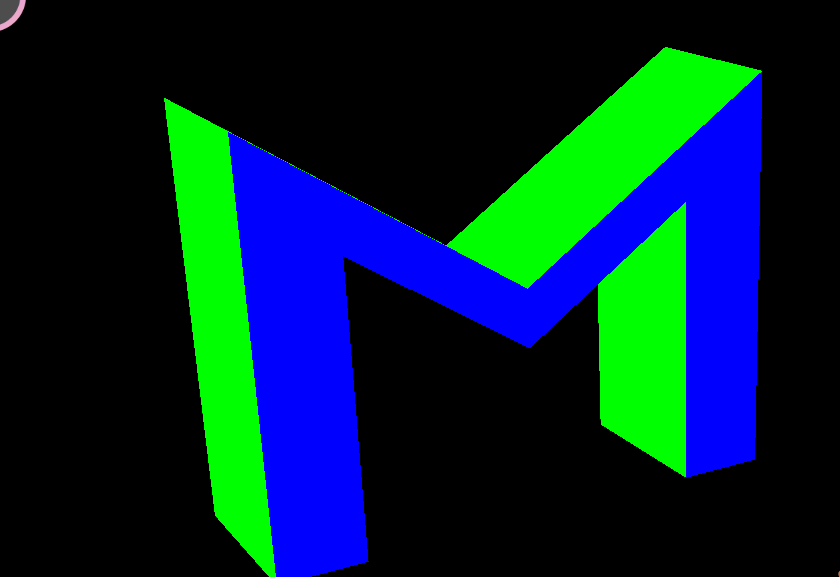
\includegraphics[width=0.4\textwidth]{img/rotate_y4.png}
    \caption{绕Y轴旋转关键帧}
    \label{fig:rotation_y}
\end{figure}

\subsubsection{Z轴旋转效果}

字母M绕Z轴旋转的关键帧序列展示旋转过程:

\begin{figure}[H]
    \centering
    
\includegraphics[width=0.4\textwidth]{img/rotate_z1.png}
    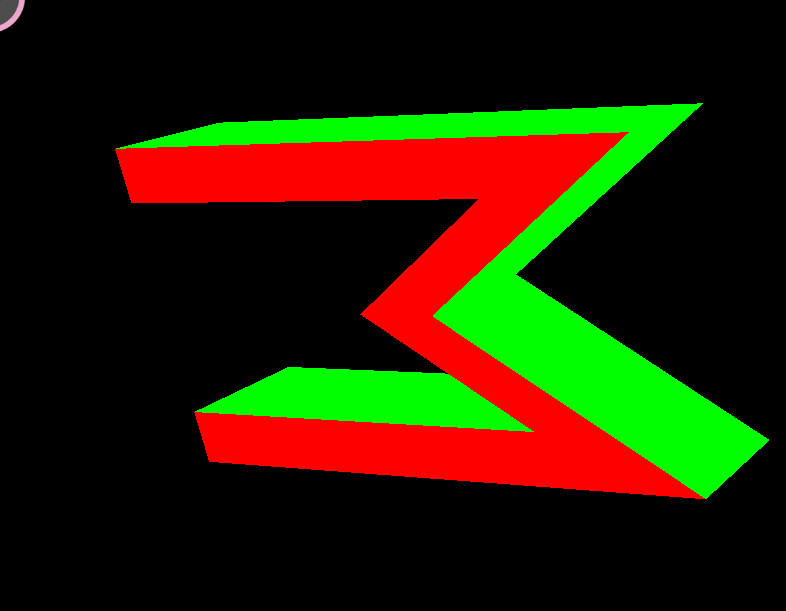
\includegraphics[width=0.4\textwidth]{img/rotate_z2.png}
    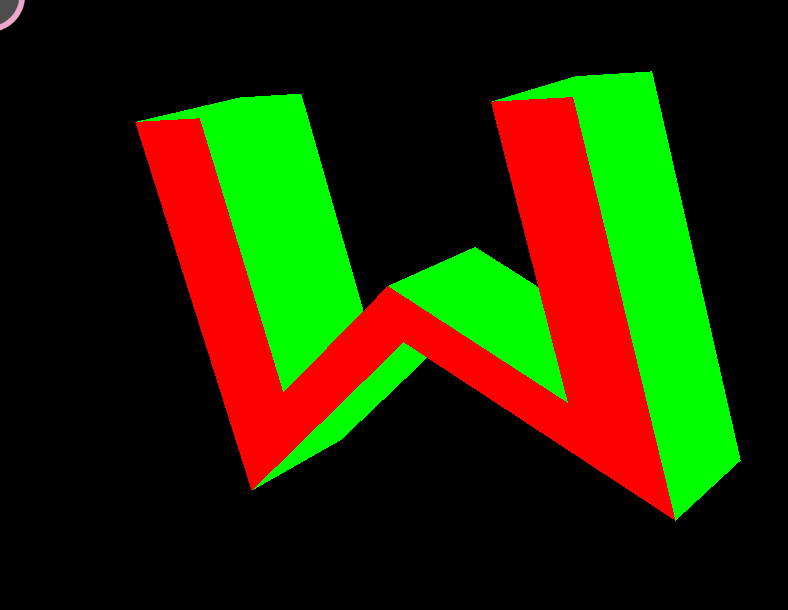
\includegraphics[width=0.4\textwidth]{img/rotate_z3.png}
    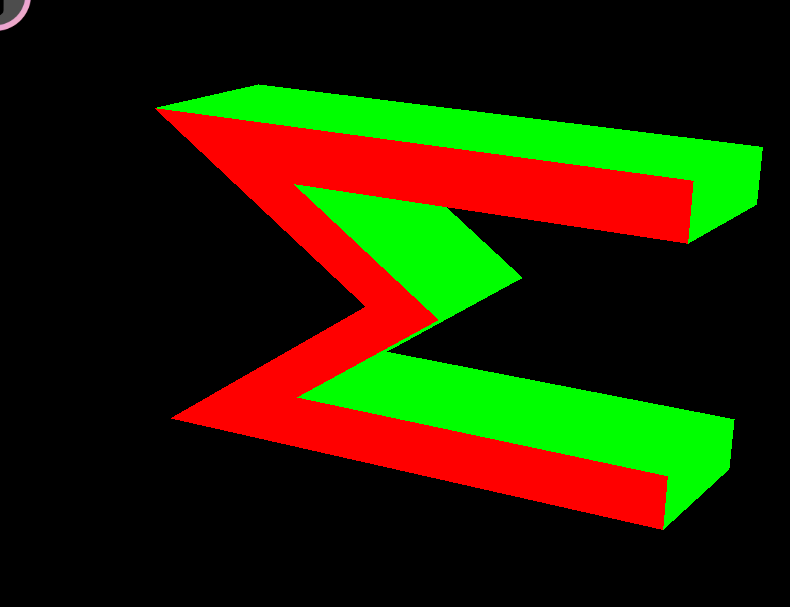
\includegraphics[width=0.4\textwidth]{img/rotate_z4.png}
    \caption{绕Z轴旋转关键帧}
    \label{fig:rotation_z}
\end{figure}

\subsubsection{旋转对比总结}

通过对比三个方向的旋转效果,可以得出以下结论:

\begin{enumerate}
    \item \textbf{X轴旋转}适合观察字母的上下结构和垂直方向的厚度变化
    \item \textbf{Y轴旋转}最能体现字母的立体感和左右侧面的厚度
    \item \textbf{Z轴旋转}保持字母正面朝向,适合展示字母在平面内的方向变化
    \item 三种旋转方式各有特点,组合使用可以全方位展示3D字母的立体结构
\end{enumerate}

\section{总结与体会}

\subsection{实验过程中的困难与解决方案}
以下是本次实验的实施过程遇到的主要困难及其解决方案：

\subsubsection{1. OpenGL环境配置问题}

\textbf{困难描述：}

初次配置OpenGL开发环境时，遇到了CMake无法找到GLFW和GLAD库的问题。

编译时出现"找不到glfw3.lib"和头文件路径错误等问题。

\textbf{解决方案：}

\begin{itemize}
    \item 仔细阅读实验指导书和CMakeLists.txt配置文件，理解第三方库的链接方式
    \item 将GLAD的头文件和源文件正确放置在项目目录中
    \item 使用绝对路径进行调试，确认路径后再改为相对路径
\end{itemize}


\subsubsection{2. 字母顶点坐标设计困难}

\textbf{困难描述：}

在设计字母M、F、Q的顶点坐标时，难以准确控制字母的形状和比例。特别是字母Q的圆形部分，使用三角形近似时效果不理想，出现明显的棱角。

\textbf{解决方案：}

\begin{itemize}
    \item 先在方格纸上手绘字母轮廓，确定关键顶点的整数坐标
    \item 对于字母Q的圆形部分，增加三角形数量以提高近似精度
    \item 使用数组存储顶点数据，便于调试和修改
    \item 编写辅助函数可视化顶点序号，方便检查三角形的连接关系
\end{itemize}

\subsubsection{3. 三维立体建模的侧面生成问题}

\textbf{困难描述：}

在从2D字母生成3D立体字母时，前后表面的生成比较简单，但侧面的自动生成遇到困难。需要识别2D轮廓的边缘，并正确连接前后表面的对应顶点，且要保证三角形的法线方向一致。

\textbf{解决方案：}

\begin{itemize}
    \item 分析2D三角形的边缘特征，提取轮廓边
    \item 为每条边缘创建两个三角形连接前后表面
    \item 使用右手法则确保法线方向朝外
    \item 通过颜色区分前面、后面和侧面，便于调试
\end{itemize}

\subsubsection{4. 二维视角图参数调节困难}

\textbf{困难描述：}

在绘制二维字母的不同视角投影图时，发现字母经常显示不完整或比例失衡，需要不断调整视野大小、投影参数和观察点位置。尤其是在切换正交与透视投影、不同视角时，参数设置稍有不当就会导致图像超出窗口或变形。

\textbf{解决方案：}

\begin{itemize}
    \item 参考OpenGL官方文档，理解glOrtho和gluPerspective各参数的实际含义
    \item 结合字母实际尺寸，合理设置视野范围和裁剪面
    \item 多次实验不同参数，记录效果，最终选取合适的参数组合
\end{itemize}

\subsection{实验收获与反思}

通过本次基于OpenGL的字母绘制实验，我在计算机图形学的理论知识和实践技能方面都获得了提升。以下是主要收获和反思：

\subsubsection{技术能力提升}

\begin{enumerate}
    \item \textbf{图形API掌握}：深入理解了OpenGL的工作原理，掌握了基本图元、顶点缓冲、变换矩阵等核心概念。能够熟练使用glBegin/glEnd进行图形绘制，理解了现代OpenGL与传统OpenGL的区别。

    \item \textbf{三维空间思维}：通过三维字母的建模和旋转实验，培养了三维空间想象能力。能够在脑海中构建物体的三维模型，理解不同视角下物体的投影效果。

    \item \textbf{算法设计能力}：实现了从2D到3D的自动建模算法，提升了几何算法的设计能力。学会了如何将复杂问题分解为简单子问题，通过模块化设计提高代码的可维护性。

    \item \textbf{调试与优化}：积累了图形程序调试的经验，学会使用颜色区分、辅助线绘制等方法定位问题。理解了顶点数据优化对性能的影响，掌握了不同绘制模式的性能差异。
\end{enumerate}

\subsubsection{理论知识深化}

\begin{enumerate}
    \item \textbf{投影变换理论}：通过实际对比正交投影和透视投影的效果，深刻理解了两种投影方式的数学原理和应用场景。认识到投影方式的选择应根据具体需求确定。

    \item \textbf{坐标系统}：系统掌握了世界坐标系、观察坐标系、裁剪坐标系等概念，理解了从模型空间到屏幕空间的完整变换流程。

    \item \textbf{图形渲染管线}：了解了OpenGL渲染管线的基本流程，理解了顶点处理、图元装配、光栅化、片段处理等阶段的作用。

    \item \textbf{性能优化原理}：通过比较不同图元类型的绘制开销，理解了顶点共享、索引缓冲等优化技术的重要性。
\end{enumerate}

\subsubsection{对计算机图形学的认识}

通过本次实验，我认识到计算机图形学是一门理论与实践紧密结合的学科，不仅需要扎实的数学基础（线性代数、几何学），还需要良好的编程能力和空间想象力。本次实验不仅让我掌握了OpenGL的基本使用方法，更重要的是培养了图形学思维方式和问题解决能力。这将成为我继续深入学习计算机图形学的坚实基础。

\subsection{实验相关的代码文件}
main\_2d.cpp: 二维字母绘制代码文件  
main\_3d.cpp: 三维字母绘制代码文件

\begin{tcolorbox}[colback=yellow!10!white, colframe=orange!75!black, title=\textbf{注意}]
运行时需要将对应的代码文件重命名为 \texttt{main.cpp}
\end{tcolorbox}

\subsection{参考资料}

\begin{enumerate}
    \item OpenGL官方文档：\url{https://www.opengl.org/documentation/}
    \item GLFW官网：\url{https://www.glfw.org/}
    \item LearnOpenGL教程：\url{https://learnopengl.com/}
    \item 《计算机图形学》教材相关章节
\end{enumerate}

\end{document}